
\chapter{Risk Based Pricing}
\section{ Preliminary definitions} 

\renewcommand{\arraystretch}{1.5} % <-- optional a
\begin{center} % <-- optional b
\[ % <-- step a
\begin{array}{|l|c|l|} \hline % <-- steps b, c; optional c, d
\mbox{Element} & \mbox{Notation}\\ \hline
\mbox{Client Interest Rate}  & r \\
\mbox{Cost of Funds Rate,Fund Transfer Pricing FTP, TT   }  & r_c \\
\mbox{Discount Rate }  & r_d\\
\mbox{Contractual Maturity }  & T \\
\hline
\end{array} % <-- step e
\] % <-- step e
\end{center}

\subsection{Default and Prepayment probabilities:}
$ \forall t \in \{1,2,...T\}$
\[ 
\begin{array}{rr} 
   p_p(t)  :&  \mbox{
   Probability that the loan will prepay at time t given that it has survived to that point } \\
   p_d(t)  : &  \mbox{
   Probability that the loan will default at time t given that it has survived to that point
   }
\end{array} \noindent
\] 

 \subsection{Survival function:}
$S(t)$ :   Probability that a loan survives until period t 
\begin{align}
S(t) & = \Pi_{s=1}^t (1-p_d(s) - p_p(s)) \\
 & = (1-p_d(1) - p_p(1))\times(1-p_d(2) - p_p(2))\times...\times(1-p_d(t) - p_p(t)) \nonumber
\end{align}

\subsection{Balance function: }
The Current Balance function $\bar{B}(t)$ is the remaining balance left at time $t-1$ for a loan with principal $B=\bar{B}(1)$ and in absence of any prepayment or default risk. For non conventional loan payments this function might not have a closed form solution. 


\paragraph{Constant installments:} The remaining balance at time $t$ for a loan with principal (Balance at t=0) B is given by 
\begin{align}
\bar{ B}(t)&=B\frac{(1+r)^T-(1+r)^{t-1}}{(1+r)^T-1}
\end{align}
\begin{align}
\bar{ I}(t)&=r\times \bar{ B}(t)
\end{align}
The acute reader will notice that the definition of $\bar{B}(t)$, in terms of the remaining balance left at time $t-1$ , was given so that we can state such a simple equation for $\bar{I}(t)$.


\paragraph{Constant amortization: } The remaining balance at time $t$ for a loan with principal (Balance at t=0) B is given by:

\begin{align}
\bar{B}(t)&=B \times (1-\frac{t-1}{T})
\end{align}


\section{ Terms included in the incremental profit (CLV)}
\subsection{ Interest on loans: }
\begin{align}
LI(t) = S(t)\bar{ B}(t)r \label{eq:li}
\end{align}
Equation (\ref{eq:li}) will be proved in section (\ref{can}). For now lets just use our intuition and state that each dollar has an unconditional probability to survive up to time $t$ of $S(t)$ 
\subsection{  Cost of Funds: }
\begin{align}
COF(t) = S_c(t)\bar{ B}_c(t)r_c
\end{align}
Where: 
\begin{align}
S_c(t)= \Pi_{s=0}^t [1- p_p(s)-(1-LGD(s))p_d(s) ]
\end{align}
The last formula can be viewed as the complement for the probability of death for 1 dollar. If a prepayment event 

\subsection{ Equity Benefit (Capital Rebate): }
\begin{align}
EB(t) = \alpha S(t)\bar{ B}(t) r_c
\end{align}

\subsection{ Fees Additional Source of revenue: }
\begin{align}
F(t) = f S(t)
\end{align}

\subsection{ Servicing Costs: }
\begin{align}
SC(t) =  \sigma S(t)
\end{align}

\subsection{ Loss from Default: }
\begin{align}
EL(t) =  p_d(t)LGD(t)S(t)\bar{ B}(t) 
\end{align}
\subsection{Recovery costs}
\begin{align}
C(t) = c\times p_d(t) S(t)
\end{align}

\subsection{ Equity Capital Charge: }
\begin{align}
 EC(t) =  \alpha S(t)\bar{ B}(t) r_e
\end{align}


\section{ Incremental Profit Definition (CLV): }
The net present value is given by:

\begin{align}
NPV(x(t),r,T)=\sum_{t=1}^T \frac{x(t)}{(1+r)^t}
\end{align}

\renewcommand{\arraystretch}{1.5} % <-- optional a
\begin{center} % <-- optional b
\[ % <-- step a
\begin{array}{|l|c|l|} \hline % <-- steps b, c; optional c, d
\mbox{Element} & \mbox{Notation} & \mbox{Calculation}\\ \hline
\mbox{Lending Interest }  & LI & NVP(LI(t),r_d,T)\\
\mbox{Cost of Funds   }  & COF & NVP(COF(t),r_d,T)\\
\mbox{Equity benefit }  & EB & NVP(EB(t),r_d,T)\\
\mbox{Fees }  & LI & NVP(F(t),r_d,T)\\
\mbox{Ancillary profit }  & A & -\\
\mbox{Origination cost}  & OC & -\\
\mbox{Commision  }  & COM & -\\
\mbox{Servicing Costs}  & SC & NVP(SC(t),r_d,T)\\
\mbox{Expected Loss }  & EL & NVP(EL(t),r_d,T)\\
\mbox{Collection costs }  & C & NVP(C(t),r_d,T)\\
\mbox{Equity charge}  & EC & NVP(EC(t),r_d,T)\\

\hline
\end{array} % <-- step e
\] % <-- step e
\end{center}

\renewcommand{\arraystretch}{1.5} % <-- optional a
\begin{center} % <-- optional b
\[ % <-- step a
\begin{array}{|l|c|l|} \hline % <-- steps b, c; optional c, d
\mbox{Element} & \mbox{Notation} & \mbox{Calculation}\\ \hline
\mbox{Net Interest Income }  & NII & LI-COF+EB\\
\mbox{Total Income  }  & TI & NII+A+F\\
\mbox{Net Income before tax}  & NIBT & TI-OC-COM-SC-LD-C\\
\mbox{Net Income after tax }  & NIAT&(1-\tau)\times NIBT \\
\mbox{Incremental profit  }  & IP & NIAT-EC\\

\hline
\end{array} % <-- step e
\] % <-- step e
\end{center}

\subsection{ Incremental Profit Function: }
Define the incremental profit function as:
\begin{align}
\pi(p)=IP(p)
\end{align}
%Page on setup equations
\section{Financial Math operators}
\subsection{Constant Installments}
We can define a $c_f$ factor to compute constant installments by defining the following:
\begin{align}
    \bar{B}(1) &= \frac{c}{(1+r)}+\frac{c}{(1+r)^2}+\frac{c}{(1+r)^3}+...++\frac{c}{(1+r)^T} \nonumber\\
    &=c\delta[1+\delta+\delta^2+\delta^3+\delta^4+...+\delta^{T-1}] \nonumber \\
    &=c\delta\left[\frac{1}{1-\delta}-\delta^T\frac{1}{1-\delta}\right] =c\delta\left(\frac{1-\delta^T}{1-\delta}\right)
\end{align}
\begin{align}
    c=\bar{B}(1)\left(\frac{1-\delta}{\delta}\right)\frac{1}{1-\delta^T}=B(1)\left[r\frac{(1+r)^T}{(1+r)^T-1}\right]
\end{align}

\begin{align}
    c_f(r,T):=\frac{r(1+r)^T}{(1+r)^T-1} \implies c:=\bar{B}(1)c_f(r,T)
\end{align}
Balance factor:
\begin{align}
    \bar{B}(t)=\bar{B}(1)\left[ \frac{(1+r)^T-(1+r)^{t-1}}{(1+r)^T-1} \right]
\end{align}
\begin{align}
    B_f(t,r,T)=\left[ \frac{(1+r)^T-(1+r)^{t-1}}{(1+r)^T-1} \right] \implies \bar{B}(t)=\bar{B}(1)B_f(t,r,T)
\end{align}
\begin{align}
    \bar{I}(t) = r\bar{B}(1)B_f(t,r,T)
\end{align}
Amortization factor:
\begin{align}
    A_f(t,r,T) &= c_f(r,T)-rB_f(t,r,T)\\
    &=\frac{r(1+r)^{t-1}}{(1+r)^T-1}
\end{align}


\begin{theorem}{1.1 (Telescopic Amortizations)}{} \label{teo:1}
Let
\[
\prod^{t-1}_{s=1}(1-A(1,r,T-s+1))=1-\sum^{t-1}_{s=1}A(s,r,T)
\]
\end{theorem}

\begin{proof}{}{} Lets define
\[
E_1=\prod^{t-1}_{s=1}(1-A(1,r,T-s+1)), \\
E_2 =1-\sum^{t-1}_{s=1}A(s,r,T)
\]
and
\[
\delta =1/(1+r)
\]
Working on $E_1$ and defining $\xi=1+r$:
\begin{align}
1-A(1,r,T-s+1) = \frac{(1+r)^{T-s+1}-1-r}{(1+r)^{T-s+1}-1}=\frac{\xi^{T-s+1}-\xi}{\xi^{T-s+1}-1} \nonumber
\end{align}

\begin{align}
\implies E_1 =& \frac{(\xi^T-\xi)}{(\xi^T-1)}\times \frac{(\xi^{T-1}-\xi)}{(\xi^{T-1}-1)} \times \frac{(\xi^{T-2}-\xi)}{(\xi^{T-2}-1)} \times ... \times \frac{(\xi^{T-t+1}-\xi)}{(\xi^{T-t+1}-1)} \nonumber\\
=&\xi^t \frac{(\xi^{T-1}-1)}{(\xi^T-1)}\times \frac{(\xi^{T-2}-1)}{(\xi^{T-1}-1)} \times \frac{(\xi^{T-3}-1)}{(\xi^{T-2}-1)} \times ... \times \frac{(\xi^{T-t}-1)}{(\xi^{T-t+1}-1)} \nonumber\\
=&\frac{\xi^T-\xi^t}{\xi^T-1} \label{eq:e1}
\end{align}

Working on $E_2$:
\begin{align}
A(s,r,T) = \frac{r(1+r)^{s-1}}{(1+r)^{T}-1}=(\xi-1)\frac{\xi^{s-1}}{\xi^{T}-1} \nonumber
\end{align}

\begin{align}
\implies E_2 =& 1-\frac{(\xi-1)(1+\xi+\xi^2+\xi^3+...+\xi^{t-1})}{\xi^T-1}\nonumber\\
=&\frac{\xi^T-\xi^t}{\xi^T-1} 
\end{align}
$\therefore E1=E2$
\end{proof}

%  Page on setup examples
\section{Alternative setups for Incremental Profit computation}



\subsection{Canonical model \label{can}} 
\begin{figure}[H]
  \centering
      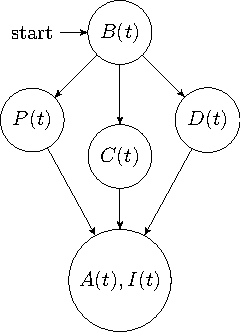
\includegraphics[width=.3\textwidth]{Graph2.pdf} 
 \caption{Graph for computations}
 \label{fig:graph2}
\end{figure}

\begin{center} % <-- optional b
\[ % <-- step a
\begin{array}{|l|c|l|} \hline % <-- steps b, c; optional c, d
\mbox{Variable} &\mbox{Notation} & \mbox{Calculation}\\ \hline
\mbox{Balance in presence of risk }  & B(t)  & B(t)\\
\mbox{Default  }  & D(t) & p_d(t) B(t)\\
\mbox{Full Prepayment}  & C(t) & p_c(t) B(t)\\
\mbox{Prepayment  }  & P(t) & p_p(t)B(t)\\
\mbox{Amortization}  & A(t) &(1-p_d(t)-p_c(t)-p_p(t)) B(t)A_f(1,r,T-t+1))\\
\mbox{Interest }  & I(t) & (1-p_d(t)-p_c(t)-p_p(t))B(t)r\\
\mbox{Principal   }  &  B(1) & B\\
\hline
\end{array} % <-- step e
\] % <-- step e
\end{center}

Notice that we defined $B(t)$ as the Loan Balance subject to risk (Conductual affected Loan Balance), as opposed to $\bar{B}(t)$, which is the Risk Free Loan Balance (Contractual Balance).  Given this definitions we can compute the recursive form for the balance function $B(t)$
\begin{align}
B(t+1) =& B(t)[1-p_d(t)-p_c(t)-p_p(t)-(1-p_d(t)-p_c(t)-p_p(t))A(1,r,T-t+1) ] \nonumber\\
     =&
    B(t)(1-p_d(t)-p_c(t)-p_p(t))(1-A(1,r,T-t+1)) \label{eq:bbar1}\
\end{align}
Notice that (\ref{eq:bbar1}) is a first order equation in difference which can be easily solved as.
\begin{align}
    B(t) =\prod^{t-1}_{s=1} (1-A(1,r,T-s+1))(1-p_d(s)-p_c(s)-p_p(s))B
\end{align}
Using theorem (\ref{teo:1}) we can state the conductual balance $B(t)$ as a function of the contractual balance.
\begin{align}
    B(t) &=\prod^{t-1}_{s=1} (1-p_d(s)-p_c(s)-p_p(s))\bar{B}(t) \nonumber\\
    &=S(t)\bar{B}(t)
\end{align}

\subsection{Prepayment dependent on initial balance}
\begin{figure}[H]
  \centering
      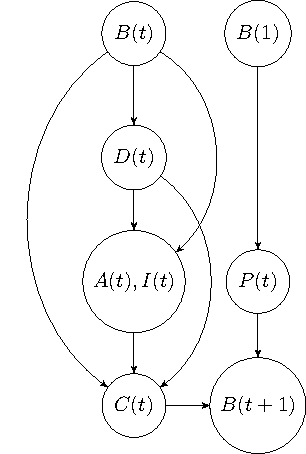
\includegraphics[width=.3\textwidth]{Graph1.pdf} 
 \caption{Topological Sort for computations}
 \label{fig:Test}
\end{figure}

\begin{center} % <-- optional b
\[ % <-- step a
\begin{array}{|l|c|l|} \hline % <-- steps b, c; optional c, d
\mbox{Variable} &\mbox{Notation} & \mbox{Calculation}\\ \hline
\mbox{Balance in presence of risk }  & B(t)  & B(t)\\
\mbox{Default  }  & D(t) & p_d(t) B(t)\\
\mbox{Amortization}  & A(t) &(1-p_d(t)) B(t)A(1,r,T-t+1))\\
\mbox{Interest }  &  I(t) & (1-p_d(t))B(t)r\\
\mbox{Full Prepayment}  & C(1) & p_c(t) B(t)[1-p_d(t)-(1-p_d(t))A(1,r,T-t+1)]\\
\mbox{Principal   }  &  B(1) & B\\
\mbox{Prepayment  }  & P(t) & p_p(t)B\\
\hline
\end{array} % <-- step e
\] % <-- step e
\end{center}

  Given this definitions we can compute the recursive form for the balance function $B(t)$
\begin{align}
\scriptstyle
     \bar{B}(t+1) =&\scriptstyle \bar{B}(t)[1-p_d(t)-p_c(t)(1-p_d(t)-(1-p_d(t))A(1,r,T-t+1))-(1-p_d(t))A(1,r,T-t+1) ]-p_p(t) \bar{B}(1) \nonumber\\
    =&\scriptstyle \bar{B}(t)[1-p_d(t)-p_c(t)+p_d(t)p_c(t)+p_c(t)(1-p_d(t)A(1,r,T-t+1)-(1-p_d(t))A(1,r,T-t+1)]
    -p_p(t) \bar{B}(1) \nonumber\\
    =&\scriptstyle
    \bar{B}(t)[ (1-p_d(t))(1-p_c(t))-(1-p_d(t))(1-p_c(t))A(1,r,T-t+1)]
    -p_p(t) \bar{B}(1) \nonumber\\
     =&\scriptstyle
    \bar{B}(t)(1-p_d(t))(1-p_c(t))(1-A(1,r,T-t+1))
    -p_p(t) \bar{B}(1) \label{eq:bbar}\
\end{align}
Notice that (\ref{eq:bbar}) is a first order equation in difference which can be easily solved as.
\begin{align}
    B(t) =\prod^{t-1}_{s=1} (1-A(1,r,T-s+1))(1-p_d(s))(1-p_p(s))B-\sum (\prod a_s) b_k
\end{align}
Using theorem (\ref{teo:1}) we can state the conductual balance $B(t)$ as a function of the contractual balance.
\begin{align}
    B(t) &=\prod^{t-1}_{s=1} (1-p_d(s))(1-p_p(s))\bar{B}(t)-\sum (\prod a_s) b_k \nonumber\\
    &=S(t)\bar{B}(t)-\sum (\prod a_s) b_k 
\end{align}
